%----------------------------------------------------------------------------------------
%	INPUT REFERENCE VOLTAGE AND POWER CONTROL.
%----------------------------------------------------------------------------------------
\subsection{Input reference voltage \& power control}


\begin{figure}[H]
\centering
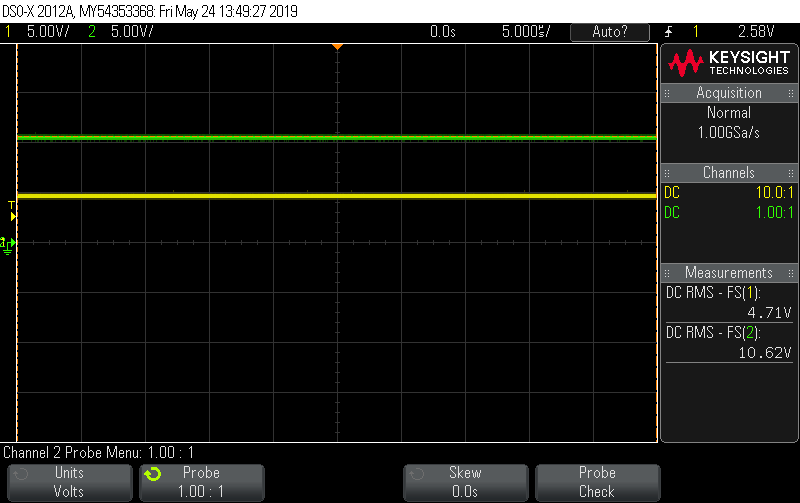
\includegraphics[width=.9\textwidth]{figures/scope_13.png}
\caption{Input reference voltage with variable resistor R6 on 100\%. The input 'OP-AMP O/P' in yellow and the output 'TP3' (input power control) in green.}
\label{fig:scope_13}
\end{figure}


\begin{figure}[H]
\centering
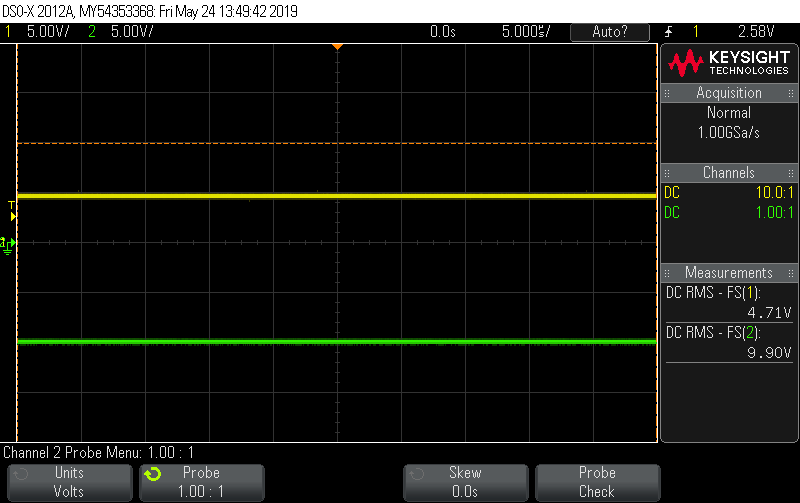
\includegraphics[width=.9\textwidth]{figures/scope_14.png}
\caption{Input reference voltage with variable resistor R6 on 0\%. The input 'OP-AMP O/P' in yellow and the output 'TP3' (input power control) in green.}
\label{fig:scope_14}
\end{figure}


\begin{figure}[H]
\centering
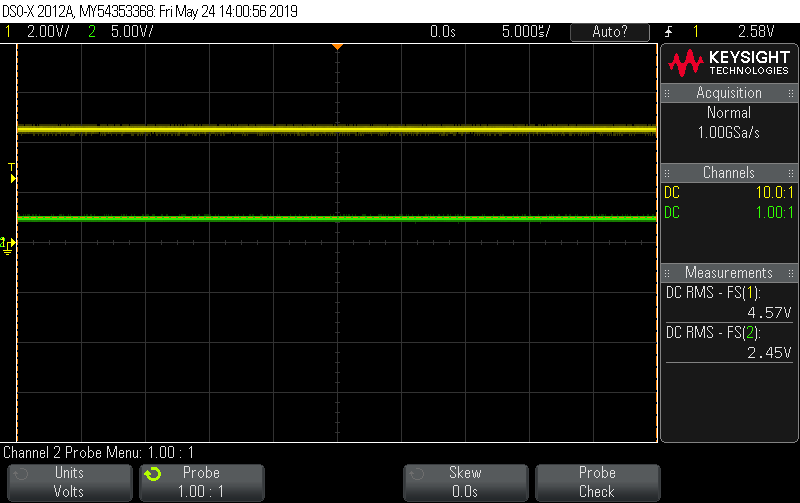
\includegraphics[width=.9\textwidth]{figures/scope_15.png}
\caption{Input reference voltage of $\SI{2.45}{\volt}$, measured in green at the positive input of the op-amp U3A. The input voltage on the negative input 'OP-AMP O/P' is $\SI{4.6}{\volt}$. The output 'TP3' is shown in yellow. It can be seen that the gain is approximately 1.}
\label{fig:scope_15}
\end{figure}

